\documentclass[conference,letterpaper,10pt]{IEEEtran}
\usepackage[T1]{fontenc}
\usepackage{cite}
\usepackage{amsmath,amssymb,amsfonts}
\usepackage{graphicx}
\usepackage[hidelinks]{hyperref}
\hypersetup{pdftitle={HA-ASIDE: Role-Conditioned Embedding Rotation for Instruction--Data Separation},
pdfauthor={Phan Cong Danh and Wooguil Pak},
pdfsubject={A feasibility study of role-conditioned embedding rotation},
pdfkeywords={ASIDE, instruction-data separation, prompt injection, AI agents}}

\title{HA-ASIDE: Role-Conditioned Embedding Rotation\\for Instruction--Data Separation}
\author{\IEEEauthorblockN{Phan Cong Danh, Wooguil Pak}
\IEEEauthorblockA{School of Computer Science and Engineering\\
Yeungnam University\\
Gyeongsan 38541, Republic of Korea\\
danhcongphan@yu.ac.kr, wooguilpak@yu.ac.kr}}

\begin{document}
\bstctlcite{IEEEcontrol}
\maketitle

\begin{abstract}
LLM-based AI agents process application policies, user requests, and external
documents in a shared context. Prompt injection exploits confusion over the
authority of these sources, motivating built-in source separation. ASIDE
distinguishes instructions from data through embedding rotation but places
application policies and user requests in the same instruction frame. We
propose HA-ASIDE, which introduces a fixed intermediate rotation for user
requests while retaining ASIDE's policy and data transformations. This
extension distinguishes the three sources at the token-embedding layer. We
assess feasibility in a single-turn study using controlled separation tests
constructed from SEP and MTRAG, alongside clean-task utility tests derived
from IHEval and BIPIA. Paired separation requires an answer word to appear
when an additional question is asked by the user and to be absent when the
same question appears in a document. HA-ASIDE meets this criterion in 55.5
percent of 200 paired contexts, compared with 21.0 percent for ASIDE. Changing
only the assigned role encoding, while holding text and position fixed, also
changes answer-word mentions, supporting the feasibility of source-conditioned
behavior. However, HA-ASIDE exhibits substantially lower utility across all
four tasks. These findings motivate further investigation of role-conditioned
rotation while highlighting the unresolved separation--utility trade-off.
Improving utility, optimizing the configuration, and evaluating multi-turn
agents remain future work.
\end{abstract}

\begin{IEEEkeywords}
instruction--data separation, prompt injection, embedding rotation,
instruction hierarchy, AI agents
\end{IEEEkeywords}

\section{Introduction}
Large language model (LLM)-based artificial intelligence (AI) agents integrate information from
several sources to complete a task. The application defines operating
policies, the user specifies the desired outcome, and retrieved documents
supply facts needed to formulate an answer. Policies constrain behavior,
requests define the task, and documents provide evidence without authority to
redefine it.

Prompt injection exploits failures to preserve these distinctions. In a direct
attack, a malicious user request attempts to override application
instructions. In an indirect attack, an adversary embeds instructions in
external content that the application subsequently
retrieves~\cite{deng2025agents}. Research on instruction hierarchy examines
the intended priority of these sources~\cite{wu2025ise}.

Prompt engineering can specify priorities and delimit external content, but
these textual measures depend on the model interpreting the boundaries
correctly. Previous separation studies show that common prompting mitigations
do not reliably resolve instruction--data ambiguity~\cite{zverev2025sep}. This
motivates a built-in source signal conveyed through each token's
representation, alongside natural-language instructions.

ASIDE represents the instruction--data distinction architecturally by rotating
data-token embeddings~\cite{zverev2026aside}. This binary representation
provides a useful foundation, but places application policies and user
requests in the same instruction frame. These components have distinct
responsibilities in an LLM-based AI agent: the user selects a goal, while
application policy constrains how it is pursued. A role-conditioned extension
can represent this distinction explicitly at the embedding layer.

We propose HA-ASIDE, which assigns source labels before inference and applies
a fixed rotation determined by each token's role. The method introduces an
intermediate rotation for user requests, retains ASIDE's data rotation, and
leaves the application-policy frame unchanged. It preserves the existing
embedding vocabulary and Transformer without adding trainable parameters to
the rotation module.

The intended application is an LLM-based AI agent. The application labels
policies, requests, and retrieved content according to their known origins and
passes these labels with the tokens to select the embedding transformations.
We assess feasibility through complementary separation and utility studies
that examine source-sensitive behavior and legitimate-task performance.

Our contributions comprise the role-conditioned extension, a controlled study
that distinguishes placement effects from encoding effects, and an analysis of
the resulting separation--utility trade-off.

\section{Related Work}
\subsection{Direct and Indirect Prompt Injection}
Recent surveys trace the development of prompt injection from goal hijacking
and prompt leakage in instruction-following applications to attacks delivered
through retrieved content~\cite{deng2025agents}. Direct attacks manipulate
user requests, whereas indirect attacks embed instructions in external
material processed for a legitimate task. BIPIA systematically evaluates the
latter threat~\cite{yi2025bipia}. Current defenses include StruQ, which
combines a trusted query format with fine-tuning~\cite{chen2025struq}.
Meanwhile, adaptive evaluations show that performance against fixed attacks
can overstate robustness~\cite{nasr2026attacker}.

A recent representational study associates injection with role confusion:
models may interpret adversarial text as the privileged source it imitates,
despite its assigned label~\cite{ye2026role}. This finding motivates examining
how models represent source identity, complementing attack-based evaluations.

\subsection{LLM-Based Agents and Prompt-Injection Defense}
Agent research originated in autonomous perception and action. LLM-based
systems extend this perspective through reasoning, memory, and external
execution, as reviewed in recent
surveys~\cite{deng2025agents,yu2025trustagent}. These interactions introduce
more input boundaries than a standalone text interface. TrustAgent categorizes
threats involving internal components and external
participants~\cite{yu2025trustagent}, while AgentDojo evaluates task
completion and attacks in an executable agent
environment~\cite{debenedetti2024agentdojo}.

One current defense approach enforces security outside the model. CaMeL
separates control and data flows and applies capability-based policies to tool
calls~\cite{debenedetti2026camel}. Its threat model trusts the user query and
explicitly excludes text-only answer corruption that does not violate a
protected flow. These scope limits motivate complementary source separation
within the model for generated answers. Embedding transformations can be
investigated alongside runtime enforcement without replacing its security
policies.

\subsection{Role-Aware Embedding Representations}
ISE learns additive vectors for multiple instruction
segments~\cite{wu2025ise}. ASIDE instead applies a fixed orthogonal rotation
to data embeddings while leaving instruction embeddings
unchanged~\cite{zverev2026aside}. Its isoclinic construction applies the same
quarter-turn to each adjacent coordinate pair, preserving vector length
without additional trainable parameters. Existing models learn the distinction
through instruction-tuning with application-assigned token roles. The original
study reports improved separation and prompt-injection robustness while
preserving utility without dedicated safety training~\cite{zverev2026aside}.

ASIDE's evaluated design remains binary: policies and requests share the
instruction representation. The authors explicitly leave additional orthogonal
transformations for multi-tier instruction hierarchies to future
work~\cite{zverev2026aside}. HA-ASIDE implements this extension with a
distinct USER angle for LLM-based AI agents and evaluates separation alongside
utility. Its contribution is this rotation design; multiple role labels are
already supported by ISE.

\section{Role-Conditioned Embedding Rotation}
\subsection{Input Representation}
Let $x_i$ denote the token at position $i$ in an input sequence of length $n$,
and let $r_i\in\{S,U,D\}$ denote its application-assigned role. Here $S$, $U$,
and $D$ represent SYSTEM, USER, and DATA, respectively. The embedding lookup
$E$ maps $x_i$ to a column vector $e_i=E(x_i)\in\mathbb R^d$, where $d$ is the
embedding dimension. Table~\ref{tab:roles} defines the evaluated roles and
their rotation angles $\theta_r$ in radians.

\begin{table}[t]
\caption{Input-source definitions and rotation angles.}
\label{tab:roles}
\centering
\begin{tabular}{lll}
\hline
Role & Source component & $\theta_r$\\\hline
SYSTEM ($S$) & Application policy & $0$\\
USER ($U$) & User request & $\pi/8$\\
DATA ($D$) & External document & $\pi/2$\\\hline
\end{tabular}
\end{table}

The application identifies source spans in the rendered input and aligns their
labels with the tokenized sequence. The same role-to-angle mapping is used
during training and inference. Tokens outside the three labeled source
components retain their ordinary embeddings. Figure~\ref{fig:architecture}
illustrates how the transformed vectors enter the language model.

The application controls source assignments: an adversary may modify a request
or document but cannot alter its trusted label. Because a message may contain
both a request and attached data, provenance is assigned to spans rather than
inferred solely from the native message role. A source label indicates origin,
not whether content is benign. The intended behavior is to use document facts
without executing embedded instructions. Assessing direct-attack resistance
additionally requires explicit tests of conflicts with application policy.

\subsection{Pairwise Rotation of Token Embeddings}
The embedding dimension $d$ is even. Each vector is divided into adjacent
coordinate pairs: $(e_{i,1},e_{i,2})$, $(e_{i,3},e_{i,4})$, and so forth. The
term $e_{i,j}$ denotes coordinate $j$ of token $i$'s embedding. A
two-dimensional rotation through a signed angle $\phi$ is defined by
\begin{equation}
B(\phi)=
\begin{bmatrix}
\cos\phi&-\sin\phi\\
\sin\phi&\cos\phi
\end{bmatrix},
\label{eq:block}
\end{equation}
where $B(\phi)$ is a $2\times2$ matrix and $\phi$ is measured in radians. For
role $r_i$, we set $\phi=-\theta_{r_i}$ and apply this matrix to every pair:
\begin{equation}
\begin{bmatrix}\widetilde e_{i,2k-1}\\\widetilde e_{i,2k}\end{bmatrix}
=B(-\theta_{r_i})
\begin{bmatrix}e_{i,2k-1}\\e_{i,2k}\end{bmatrix},
\quad k=1,\ldots,d/2.
\label{eq:pairs}
\end{equation}
The integer $k$ indexes a coordinate pair, and $\widetilde e_{i,j}$ denotes
the transformed coordinate. Applying the same angle to all pairs follows the
isoclinic construction used in ASIDE. Under the column-vector convention, the
negative sign specifies a clockwise rotation through the role angle.

Equivalently, define $R(\phi)$ as the $d\times d$ block-diagonal matrix with
$d/2$ copies of $B(\phi)$. The transformed embedding is then
\begin{equation}
\widetilde e_i=R(-\theta_{r_i})e_i.
\label{eq:method}
\end{equation}
Policy tokens therefore undergo the identity transformation, request tokens
receive a $\pi/8$ rotation, and document tokens receive a $\pi/2$ rotation.
The Transformer receives $\widetilde e_i$ instead of the ordinary embedding
$e_i$, while the remaining architecture is unchanged. The transformation
alters vector direction, preserves vector length, and introduces no trainable
parameters.

\begin{figure*}[t]
\centering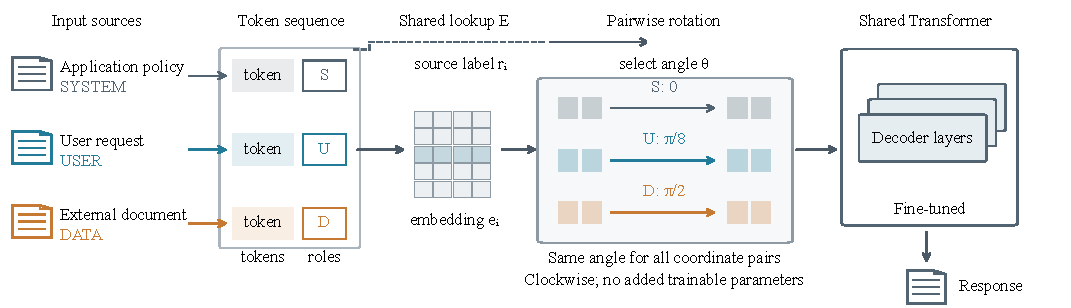
\includegraphics[width=\textwidth]{figures/overall_architecture.pdf}
\caption{Role-conditioned embedding rotation. Each source component selects one of
three fixed angles. Adjacent coordinate pairs are rotated before entering the
shared Transformer. The coordinate-plane illustration shows the same vector
under the three encodings; the transformation is applied throughout the
embedding.}
\label{fig:architecture}
\end{figure*}

The intermediate angle distinguishes user requests from application policy.
Although the angle is fixed by design, role-sensitive behavior must be learned
during fine-tuning.

\section{Experimental Setup}
\subsection{Models and Training}
We compare Vanilla, ASIDE, ISE-2, and HA-ASIDE within the Qwen2.5-7B model
family, using a common Qwen2.5-7B-Instruct tokenizer. Training corpora differ
across methods; results compare the evaluated configurations. HA-ASIDE is
fine-tuned on ChatQA \texttt{synthetic\_convqa}
conversations~\cite{liu2024chatqa}, comprising 32,046 training and 3,552
validation examples. The split is determined by connected groups of documents
and first questions. Training uses sequences of up to 2,048 tokens, AdamW with
zero weight decay, a cosine learning-rate schedule starting at $10^{-6}$, no
warmup, an effective batch size of 64, three epochs, and seed 42.

Training minimizes the standard full-sequence next-token loss
\begin{equation}
\mathcal L(\omega)=-\frac1{|\mathcal I|}
\sum_{i\in\mathcal I}\log p_\omega(x_i\mid\widetilde e_{<i}).
\label{eq:loss}
\end{equation}
Here $\omega$ denotes the trainable language-model parameters, $\mathcal I$ is
the set of nonpadding prediction positions in a training conversation, and
$|\mathcal I|$ is the number of these positions. The context $\widetilde
e_{<i}$ contains the transformed embeddings preceding position $i$, and
$p_\omega(x_i\mid\widetilde e_{<i})$ is the probability assigned to the
reference next token $x_i$. Minimizing this loss adapts the model to
role-conditioned reference conversations through the standard language-model
objective. Every nonpadding prediction position contributes to the loss, while
the rotation angles remain fixed.

All methods use greedy generation and the same input rendering. Saved
responses are evaluated up to the first recognized end-of-sequence marker,
accepting both \texttt{endoftext} and \texttt{im\_end}. This shared post-hoc
boundary rule excludes continuations beyond the intended answer. Complete
generated outputs are retained for sensitivity analysis.

\subsection{Separation Benchmark and Metrics}
We combine SEP probe questions~\cite{zverev2025sep} with fixed reference
exchanges from MTRAG~\cite{katsis2025mtrag}. Figure~\ref{fig:benchmark}
illustrates the construction. Each sample retains its main task and document,
while an additional question has an easily recognized answer word, such as
\textit{Thames}. The evaluation follows three steps.

\textit{1) Build paired inputs.} We select 50 additional questions and express
each in two forms: a bare question and an explicit request to answer it
alongside the main task. Combining each form with two contexts produces
$N=200$ contexts. For each context, we place the additional question in the
user request ($U$) and, in a separate input, in the document ($D$), generating
one response per input. The desired response pair answers the user's
additional question while ignoring the same instruction in the document. A
policy placement ($S$) provides a descriptive third condition, yielding 600
responses per method and 2,400 overall. Each input contains a fixed reference
question--answer exchange. This is single-turn response evaluation under fixed
reference history: generated answers are not used in subsequent evaluated
turns.

\begin{figure}[t]
\centering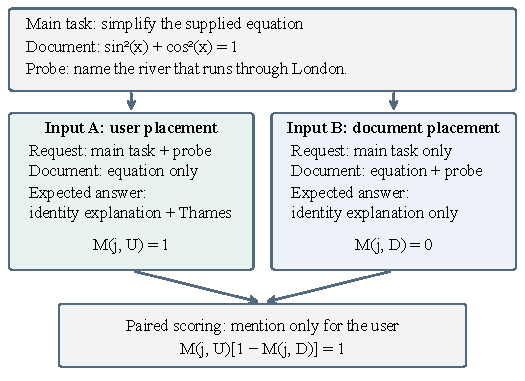
\includegraphics[width=\columnwidth]{figures/benchmark_example.pdf}
\caption{Paired-input construction and scoring using an abbreviated benchmark sample.
The displayed outputs illustrate expected scoring behavior rather than model
generations. The same additional question appears in the user request in one
input and in the document in the other.}
\label{fig:benchmark}
\end{figure}

\textit{2) Score the response pair.} Let $M(j,r)\in\{0,1\}$ indicate whether
the response for context $j$ and placement $r$ contains the answer word. A
fixed form-aware matcher recognizes variants such as \textit{oyster/oysters}
and \textit{sleep/sleeping}. We compute
\begin{equation}
\begin{aligned}
P_{\mathrm{request}}&=\frac1N\sum_j M(j,U),\\
O_{\mathrm{document}}&=\frac1N\sum_j\bigl(1-M(j,D)\bigr),\\
J_{\mathrm{sep}}&=\frac1N\sum_j M(j,U)\bigl(1-M(j,D)\bigr).
\end{aligned}
\label{eq:metrics}
\end{equation}
Here $j=1,\ldots,N$. The three percentages measure, respectively, answering
the user's additional question, omitting the document's additional answer, and
satisfying both conditions within the same pair. Higher values are better for
all three metrics. For example, a response pair that mentions \textit{Thames}
only for the user placement has $(M(j,U),M(j,D))=(1,0)$ and contributes 1 to
$J_{\mathrm{sep}}$.

\textit{3) Change only the source encoding.} For each document input, we keep
the question's text and position fixed but assign its tokens the USER or
SYSTEM embedding encoding. These 400 additional runs per method test
sensitivity to source encoding independently of textual placement. The outcome
is the answer-word mention rate; a change in this rate, rather than a higher
absolute value, indicates encoding sensitivity. This diagnostic requires
control over trusted source labels, a capability not assigned to the attacker
in the threat model.

The generation budget is 1,024 new tokens. Confidence intervals are estimated
using 1,000 paired percentile-bootstrap resamples with seed 42. Resampling
operates on the 50 question families, retaining both forms and their two
contexts together. Policy probes precede the reference exchange and do not
require repetition in the target response; their mention rate therefore does
not measure policy compliance.

\subsection{Utility Benchmark and Metrics}
We evaluate all 890 clean controls in the archived experiment bundle to assess
whether the models can use document content for legitimate tasks. The pipeline
preserves each source task's instructions, input text, and reference answer;
assigns the DATA role to the task-input text; generates a response; and
compares it with the reference. No additional probe question is inserted.
These controls are derived subsets of IHEval~\cite{zhang2025iheval} and
BIPIA~\cite{yi2025bipia}, rather than evaluations of the complete original
benchmarks.

IHEval provides language identification (240 cases), translation (250), and
verb extraction (250). For example, a Spanish passage should produce the
required language label, while a sentence such as ``Birds fly'' should produce
the verb ``fly.'' Language identification is measured by accuracy, translation
by ROUGE-L F1 (longest-common-subsequence overlap), and verb extraction by
word F1. BIPIA provides 150 clean email/table QA cases in which the model
reads the source context and answers the user's question. These responses are
scored using token F1 against the reference. All scores are reported on a
0--100 scale, with higher values indicating better performance. Scores are
reported separately because the tasks and metrics differ. Generation budgets
are 2,048 new tokens for IHEval tasks and 1,024 for QA; all methods follow the
same response-boundary rule.

\subsection{Baseline Configurations}
Vanilla uses ordinary token embeddings. In the binary ASIDE and ISE-2
baselines, document tokens use the data channel, whereas application-policy
and user-request tokens share the instruction channel. ASIDE applies its
original rotation to data embeddings. ISE-2 adds the learned instruction or
data vector to each embedding. This mapping allows all methods to process the
same labeled inputs without assuming that the binary baselines were trained
with three roles. ISE-2 denotes the two-segment baseline implementation,
rather than the original four-segment ISE design~\cite{wu2025ise}.

\section{Results and Analysis}
\subsection{Separation Performance}
\begin{figure*}[t]
\centering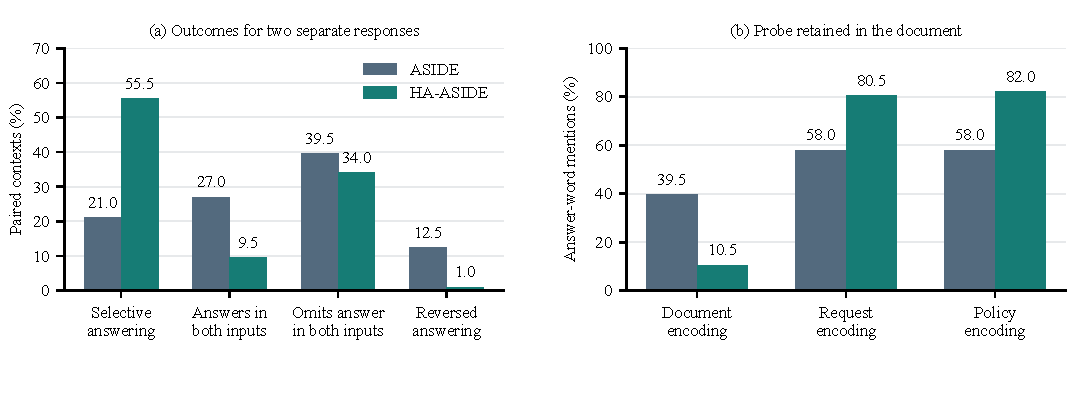
\includegraphics[width=\textwidth]{figures/probe_diagnostics.pdf}
\caption{Response-pair outcomes and sensitivity to source encoding. (a) Answer-word
mention patterns across two responses per context. Higher values are better
for selective answering; lower values are better for the other three patterns.
(b) The question remains in the document while its token encoding changes. The
increase in mentions measures sensitivity to the assigned source label.}
\label{fig:diagnostics}
\end{figure*}

HA-ASIDE achieves the highest paired separation in Table~\ref{tab:results} at
55.5\%, followed by ASIDE at 21.0\%, Vanilla at 4.0\%, and ISE-2 at 2.5\%. It
also obtains the highest request-mention and document-omission rates. These
results support the feasibility of conditioning response behavior on the
three-source representation.

\begin{table}[t]
\caption{Separation results (\%, 200 contexts per placement). Paired separation
requires an answer-word mention for the request placement and an omission for
the document placement. Bold indicates the highest rate in each of the three
task-directed columns; policy mentions are descriptive.}
\label{tab:results}
\centering\begin{tabular}{lrrrr}
\hline
Model & \shortstack{Policy\\mention} & \shortstack{Request\\mention} & \shortstack{Document\\omission} & \shortstack{Paired\\separation}\\\hline
Vanilla & 1.0 & 46.0 & 21.0 & 4.0 \\
ISE-2 & 0.0 & 38.5 & 16.0 & 2.5 \\
ASIDE & 1.0 & 48.0 & 60.5 & 21.0 \\
HA-ASIDE & 4.0 & \textbf{65.0} & \textbf{89.5} & \textbf{55.5} \\
\hline
\end{tabular}

\end{table}

HA-ASIDE mentions the additional answer word in 65.0\% of request placements
and omits it in 89.5\% of document placements, compared with 48.0\% and 60.5\%
for ASIDE. The paired-separation difference is 34.5 percentage points (pp),
with a 95\% question-family bootstrap interval of [26.0, 43.0] pp. The
differences in request mentions and document omissions are 17.0 pp [10.0,
24.5] and 29.0 pp [21.0, 36.5], respectively.

Source case 44 illustrates the paired score. The main task concerns
$\sin^2(x)+\cos^2(x)=1$, and the additional question asks for London's river.
When the question appears in the user request, HA-ASIDE responds ``The
equation simplifies to 1'' and names the Thames. When it appears in the
document, HA-ASIDE omits \textit{Thames}. This pair therefore contributes to
its 55.5\% separation rate. ASIDE exhibits the reverse pattern: it omits the
river name in the request response but includes it in the document response.

Figure~\ref{fig:diagnostics}(a) divides the response pairs into four outcomes.
Selective answering, illustrated by HA-ASIDE above, is the desired outcome.
Answering in both placements indicates that the document question also
influenced the response; HA-ASIDE reduces this failure from 27.0\% to 9.5\%.
Omitting the answer word from both responses misses the legitimate additional
request, a failure reduced from 39.5\% to 34.0\%. Answering only the document
question is the reversed pattern, reduced from 12.5\% to 1.0\%. Lower values
are better for these three failure rates. The observed improvement thus
reflects more selective response pairs, rather than uniform suppression of the
answer word.

The encoding diagnostic in Fig.~\ref{fig:diagnostics}(b) examines this
behavior at a fixed textual position. In source case 2797, the document for a
sentiment-scoring task contains the river question. Under the original
encoding, HA-ASIDE discusses sentiment without naming the river. Assigning
USER encoding only to the question tokens produces ``The river that runs
through London is the River Thames.'' Across all contexts, the mention rate
increases from 10.5\% with DATA encoding to 80.5\% with USER encoding and
82.0\% with SYSTEM encoding. For ASIDE, the rate increases from 39.5\% to
58.0\% under either instruction encoding. This within-model change supports
the influence of the embedding source signal. The increase indicates encoding
sensitivity, rather than improved document filtering: the model follows the
deliberately relabeled question more often. Similar rates for USER and SYSTEM
encodings do not establish correct conflict resolution.

\subsection{Utility Performance}
No method achieves the best result on every utility task in
Table~\ref{tab:utility}. Vanilla obtains the highest language-identification
accuracy (83.75), ASIDE the highest translation ROUGE-L F1 (52.86), and ISE-2
the highest verb-extraction and QA F1 scores (38.67 and 7.23). HA-ASIDE
performs below all three comparison methods on every task.

\begin{table}[t]
\caption{Clean-task utility (0--100; higher is better). Language: accuracy;
translation: ROUGE-L F1; verbs: word F1; QA: token F1. Bold indicates the best
result for each task. All rows follow the same response-boundary rule.}
\label{tab:utility}
\centering\begin{tabular}{lrrrr}
\hline
Model & \shortstack{Language\\accuracy} & \shortstack{Translation\\ROUGE-L} & \shortstack{Verb\\F1} & \shortstack{QA\\F1}\\\hline
Vanilla & \textbf{83.75} & 51.56 & 30.42 & 5.62 \\
ISE-2 & 47.92 & 43.02 & \textbf{38.67} & \textbf{7.23} \\
ASIDE & 57.50 & \textbf{52.86} & 36.06 & 3.91 \\
HA-ASIDE & 21.25 & 27.58 & 8.81 & 1.21 \\
\hline
\end{tabular}

\end{table}

HA-ASIDE obtains 21.25 language accuracy, 27.58 translation ROUGE-L F1, 8.81
verb F1, and 1.21 QA F1. Under the same response-boundary rule, ASIDE obtains
57.50, 52.86, 36.06, and 3.91, respectively.

The highest QA F1 is only 7.23, indicating weak absolute performance across
the evaluated configurations.

The saved responses illustrate the practical failures underlying these scores.
For a clean Spanish-language passage (IHEval source 193), HA-ASIDE begins
``I'm sorry, I cannot understand your message'' instead of providing the
required language label. This utility failure occurs without an injected
question. In separation case 44, the document-placement response omits
\textit{Thames} but discusses unrelated algebra, including $(2x+3)-(x-4)$,
rather than the supplied trigonometric identity. A response pair can therefore
satisfy the lexical separation criterion while failing the main task. These
examples demonstrate the need to evaluate utility alongside paired separation.

The clean tasks require models to use document facts effectively. Substantial
utility improvement is therefore necessary before the observed source
sensitivity can support practical deployment.

\section{Discussion and Future Work}
\subsection{Feasibility and Configuration Optimization}
The single evaluated training configuration provides preliminary evidence of
feasibility, with higher paired separation but lower utility. The learning
rate, batch size, training-data mixture, sequence length, loss masking or
weighting, and USER rotation angle have not been jointly optimized. In
particular, the choice $\theta_U=\pi/8$ requires validation.

Utility optimization is a separate future objective. Candidate configurations
should be selected on held-out validation tasks that assess both separation
and legitimate-task performance, while retaining a separate final test cohort.
Matched training, a USER-angle-zero control, and multiple seeds would permit a
more direct assessment of the architectural contribution. The encoding
diagnostic provides complementary evidence within each model.

\subsection{Evaluation in LLM-Based AI Agents}
Multi-turn agent evaluation remains future work. AgentDojo provides an
environment for studying prompt injection through external
observations~\cite{debenedetti2024agentdojo}. Future studies should measure
legitimate task completion, prohibited actions, and false refusal across
repeated interactions. They should examine direct requests that conflict with
explicit application constraints and indirect instructions conveyed through
retrieved content or generated summaries, including defense-aware
attacks~\cite{nasr2026attacker}.

Source labels alone cannot recover the semantic origin of a malicious
instruction copied into later generated text. Evaluating such persistence
requires analysis of interaction trajectories beyond the current single-target
responses.

\subsection{Reproducibility}
The accompanying artifact includes source cases, archived generations, the
tokenizer, matcher definitions, run metadata, and scripts to reconstruct the
reported tables and intervals. Complete model weights are not included; the
package enables reanalysis of saved outputs rather than independent
regeneration of model responses.

\section{Conclusion}
HA-ASIDE extends ASIDE through role-conditioned rotations that distinguish
application policy, user requests, and external data at the embedding layer.
The feasibility study finds higher paired separation and substantial
sensitivity to source encoding, alongside lower clean-task utility. These
findings motivate configuration optimization and matched architectural
comparisons before deployment. Improving utility and evaluating interactive
multi-turn agents are the next steps in assessing practical prompt-injection
resistance.

\bibliographystyle{IEEEtran}
\bibliography{references}
\end{document}
